% Created by tikzDevice version 0.12.3.1 on 2022-08-18 15:37:36
% !TEX encoding = UTF-8 Unicode
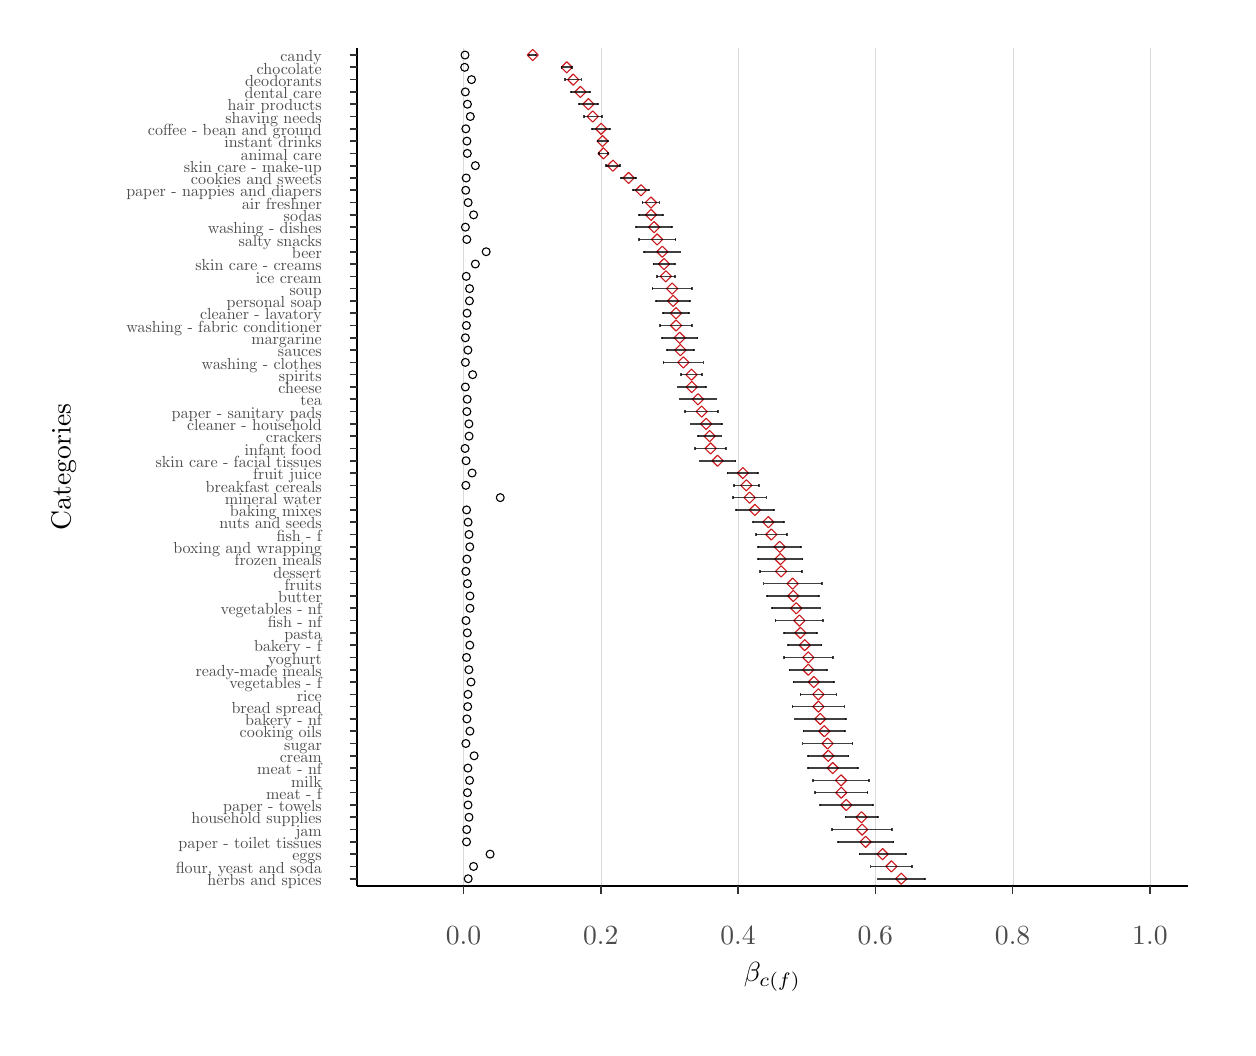
\begin{tikzpicture}[x=1pt,y=1pt]
\definecolor{fillColor}{RGB}{255,255,255}
\path[use as bounding box,fill=fillColor,fill opacity=0.00] (0,0) rectangle (433.62,361.35);
\begin{scope}
\path[clip] (  0.00,  0.00) rectangle (433.62,361.35);
\definecolor{drawColor}{RGB}{255,255,255}
\definecolor{fillColor}{RGB}{255,255,255}

\path[draw=drawColor,line width= 0.6pt,line join=round,line cap=round,fill=fillColor] (  0.00,  0.00) rectangle (433.62,361.35);
\end{scope}
\begin{scope}
\path[clip] (119.04, 51.15) rectangle (419.17,354.12);
\definecolor{drawColor}{RGB}{255,255,255}

\path[draw=drawColor,line width= 0.3pt,line join=round] (132.68, 51.15) --
	(132.68,354.12);

\path[draw=drawColor,line width= 0.3pt,line join=round] (182.29, 51.15) --
	(182.29,354.12);

\path[draw=drawColor,line width= 0.3pt,line join=round] (231.90, 51.15) --
	(231.90,354.12);

\path[draw=drawColor,line width= 0.3pt,line join=round] (281.51, 51.15) --
	(281.51,354.12);

\path[draw=drawColor,line width= 0.3pt,line join=round] (331.11, 51.15) --
	(331.11,354.12);

\path[draw=drawColor,line width= 0.3pt,line join=round] (380.72, 51.15) --
	(380.72,354.12);
\definecolor{drawColor}{gray}{0.85}

\path[draw=drawColor,line width= 0.1pt,line join=round] (157.49, 51.15) --
	(157.49,354.12);

\path[draw=drawColor,line width= 0.1pt,line join=round] (207.09, 51.15) --
	(207.09,354.12);

\path[draw=drawColor,line width= 0.1pt,line join=round] (256.70, 51.15) --
	(256.70,354.12);

\path[draw=drawColor,line width= 0.1pt,line join=round] (306.31, 51.15) --
	(306.31,354.12);

\path[draw=drawColor,line width= 0.1pt,line join=round] (355.92, 51.15) --
	(355.92,354.12);

\path[draw=drawColor,line width= 0.1pt,line join=round] (405.52, 51.15) --
	(405.52,354.12);
\definecolor{drawColor}{RGB}{0,0,0}

\path[draw=drawColor,line width= 0.4pt,line join=round,line cap=round] (159.15,298.15) circle (  1.43);

\path[draw=drawColor,line width= 0.4pt,line join=round,line cap=round] (158.86,315.92) circle (  1.43);

\path[draw=drawColor,line width= 0.4pt,line join=round,line cap=round] (159.76,138.22) circle (  1.43);

\path[draw=drawColor,line width= 0.4pt,line join=round,line cap=round] (158.71,111.57) circle (  1.43);

\path[draw=drawColor,line width= 0.4pt,line join=round,line cap=round] (158.60,187.09) circle (  1.43);

\path[draw=drawColor,line width= 0.4pt,line join=round,line cap=round] (165.68,280.38) circle (  1.43);

\path[draw=drawColor,line width= 0.4pt,line join=round,line cap=round] (159.75,173.76) circle (  1.43);

\path[draw=drawColor,line width= 0.4pt,line join=round,line cap=round] (159.00,116.01) circle (  1.43);

\path[draw=drawColor,line width= 0.4pt,line join=round,line cap=round] (158.33,195.97) circle (  1.43);

\path[draw=drawColor,line width= 0.4pt,line join=round,line cap=round] (159.82,155.99) circle (  1.43);

\path[draw=drawColor,line width= 0.4pt,line join=round,line cap=round] (158.03,351.46) circle (  1.43);

\path[draw=drawColor,line width= 0.4pt,line join=round,line cap=round] (158.15,231.51) circle (  1.43);

\path[draw=drawColor,line width= 0.4pt,line join=round,line cap=round] (157.91,347.02) circle (  1.43);

\path[draw=drawColor,line width= 0.4pt,line join=round,line cap=round] (159.44,218.19) circle (  1.43);

\path[draw=drawColor,line width= 0.4pt,line join=round,line cap=round] (158.76,258.17) circle (  1.43);

\path[draw=drawColor,line width= 0.4pt,line join=round,line cap=round] (158.32,324.80) circle (  1.43);

\path[draw=drawColor,line width= 0.4pt,line join=round,line cap=round] (158.45,307.03) circle (  1.43);

\path[draw=drawColor,line width= 0.4pt,line join=round,line cap=round] (159.80,107.13) circle (  1.43);

\path[draw=drawColor,line width= 0.4pt,line join=round,line cap=round] (159.50,213.74) circle (  1.43);

\path[draw=drawColor,line width= 0.4pt,line join=round,line cap=round] (161.32, 98.24) circle (  1.43);

\path[draw=drawColor,line width= 0.4pt,line join=round,line cap=round] (158.14,338.13) circle (  1.43);

\path[draw=drawColor,line width= 0.4pt,line join=round,line cap=round] (160.39,342.57) circle (  1.43);

\path[draw=drawColor,line width= 0.4pt,line join=round,line cap=round] (158.34,164.88) circle (  1.43);

\path[draw=drawColor,line width= 0.4pt,line join=round,line cap=round] (167.09, 62.70) circle (  1.43);

\path[draw=drawColor,line width= 0.4pt,line join=round,line cap=round] (159.47,178.21) circle (  1.43);

\path[draw=drawColor,line width= 0.4pt,line join=round,line cap=round] (158.38,147.11) circle (  1.43);

\path[draw=drawColor,line width= 0.4pt,line join=round,line cap=round] (161.12, 58.26) circle (  1.43);

\path[draw=drawColor,line width= 0.4pt,line join=round,line cap=round] (158.70,169.32) circle (  1.43);

\path[draw=drawColor,line width= 0.4pt,line join=round,line cap=round] (160.59,200.42) circle (  1.43);

\path[draw=drawColor,line width= 0.4pt,line join=round,line cap=round] (158.90,160.44) circle (  1.43);

\path[draw=drawColor,line width= 0.4pt,line join=round,line cap=round] (158.91,333.69) circle (  1.43);

\path[draw=drawColor,line width= 0.4pt,line join=round,line cap=round] (159.18, 53.82) circle (  1.43);

\path[draw=drawColor,line width= 0.4pt,line join=round,line cap=round] (159.47, 76.03) circle (  1.43);

\path[draw=drawColor,line width= 0.4pt,line join=round,line cap=round] (158.47,271.49) circle (  1.43);

\path[draw=drawColor,line width= 0.4pt,line join=round,line cap=round] (158.04,209.30) circle (  1.43);

\path[draw=drawColor,line width= 0.4pt,line join=round,line cap=round] (158.72,320.36) circle (  1.43);

\path[draw=drawColor,line width= 0.4pt,line join=round,line cap=round] (158.65, 71.59) circle (  1.43);

\path[draw=drawColor,line width= 0.4pt,line join=round,line cap=round] (158.16,249.28) circle (  1.43);

\path[draw=drawColor,line width= 0.4pt,line join=round,line cap=round] (158.91, 84.92) circle (  1.43);

\path[draw=drawColor,line width= 0.4pt,line join=round,line cap=round] (159.07, 93.80) circle (  1.43);

\path[draw=drawColor,line width= 0.4pt,line join=round,line cap=round] (159.67, 89.36) circle (  1.43);

\path[draw=drawColor,line width= 0.4pt,line join=round,line cap=round] (170.77,191.53) circle (  1.43);

\path[draw=drawColor,line width= 0.4pt,line join=round,line cap=round] (159.14,182.65) circle (  1.43);

\path[draw=drawColor,line width= 0.4pt,line join=round,line cap=round] (158.29,302.59) circle (  1.43);

\path[draw=drawColor,line width= 0.4pt,line join=round,line cap=round] (158.71,222.63) circle (  1.43);

\path[draw=drawColor,line width= 0.4pt,line join=round,line cap=round] (158.58, 67.15) circle (  1.43);

\path[draw=drawColor,line width= 0.4pt,line join=round,line cap=round] (159.12, 80.47) circle (  1.43);

\path[draw=drawColor,line width= 0.4pt,line join=round,line cap=round] (158.85,142.67) circle (  1.43);

\path[draw=drawColor,line width= 0.4pt,line join=round,line cap=round] (159.63,262.61) circle (  1.43);

\path[draw=drawColor,line width= 0.4pt,line join=round,line cap=round] (159.44,129.34) circle (  1.43);

\path[draw=drawColor,line width= 0.4pt,line join=round,line cap=round] (159.11,120.45) circle (  1.43);

\path[draw=drawColor,line width= 0.4pt,line join=round,line cap=round] (158.68,284.82) circle (  1.43);

\path[draw=drawColor,line width= 0.4pt,line join=round,line cap=round] (159.07,244.84) circle (  1.43);

\path[draw=drawColor,line width= 0.4pt,line join=round,line cap=round] (159.94,329.25) circle (  1.43);

\path[draw=drawColor,line width= 0.4pt,line join=round,line cap=round] (161.77,275.94) circle (  1.43);

\path[draw=drawColor,line width= 0.4pt,line join=round,line cap=round] (158.40,204.86) circle (  1.43);

\path[draw=drawColor,line width= 0.4pt,line join=round,line cap=round] (161.77,311.48) circle (  1.43);

\path[draw=drawColor,line width= 0.4pt,line join=round,line cap=round] (161.14,293.71) circle (  1.43);

\path[draw=drawColor,line width= 0.4pt,line join=round,line cap=round] (159.68,267.05) circle (  1.43);

\path[draw=drawColor,line width= 0.4pt,line join=round,line cap=round] (160.79,235.96) circle (  1.43);

\path[draw=drawColor,line width= 0.4pt,line join=round,line cap=round] (158.34,102.69) circle (  1.43);

\path[draw=drawColor,line width= 0.4pt,line join=round,line cap=round] (158.82,227.07) circle (  1.43);

\path[draw=drawColor,line width= 0.4pt,line join=round,line cap=round] (160.20,124.90) circle (  1.43);

\path[draw=drawColor,line width= 0.4pt,line join=round,line cap=round] (159.82,151.55) circle (  1.43);

\path[draw=drawColor,line width= 0.4pt,line join=round,line cap=round] (158.16,240.40) circle (  1.43);

\path[draw=drawColor,line width= 0.4pt,line join=round,line cap=round] (158.17,289.26) circle (  1.43);

\path[draw=drawColor,line width= 0.4pt,line join=round,line cap=round] (158.53,253.73) circle (  1.43);

\path[draw=drawColor,line width= 0.4pt,line join=round,line cap=round] (158.59,133.78) circle (  1.43);
\definecolor{drawColor}{RGB}{203,24,29}

\path[draw=drawColor,line width= 0.4pt,line join=round,line cap=round] (223.21,298.15) --
	(225.23,300.17) --
	(227.25,298.15) --
	(225.23,296.13) --
	cycle;

\path[draw=drawColor,line width= 0.4pt,line join=round,line cap=round] (206.05,315.92) --
	(208.06,317.94) --
	(210.08,315.92) --
	(208.06,313.90) --
	cycle;

\path[draw=drawColor,line width= 0.4pt,line join=round,line cap=round] (278.77,138.22) --
	(280.79,140.24) --
	(282.81,138.22) --
	(280.79,136.21) --
	cycle;

\path[draw=drawColor,line width= 0.4pt,line join=round,line cap=round] (284.38,111.57) --
	(286.40,113.59) --
	(288.42,111.57) --
	(286.40,109.55) --
	cycle;

\path[draw=drawColor,line width= 0.4pt,line join=round,line cap=round] (260.78,187.09) --
	(262.80,189.11) --
	(264.81,187.09) --
	(262.80,185.07) --
	cycle;

\path[draw=drawColor,line width= 0.4pt,line join=round,line cap=round] (227.31,280.38) --
	(229.32,282.40) --
	(231.34,280.38) --
	(229.32,278.36) --
	cycle;

\path[draw=drawColor,line width= 0.4pt,line join=round,line cap=round] (269.71,173.76) --
	(271.73,175.78) --
	(273.74,173.76) --
	(271.73,171.75) --
	cycle;

\path[draw=drawColor,line width= 0.4pt,line join=round,line cap=round] (283.72,116.01) --
	(285.74,118.03) --
	(287.75,116.01) --
	(285.74,113.99) --
	cycle;

\path[draw=drawColor,line width= 0.4pt,line join=round,line cap=round] (257.65,195.97) --
	(259.67,197.99) --
	(261.69,195.97) --
	(259.67,193.96) --
	cycle;

\path[draw=drawColor,line width= 0.4pt,line join=round,line cap=round] (274.64,155.99) --
	(276.66,158.01) --
	(278.67,155.99) --
	(276.66,153.98) --
	cycle;

\path[draw=drawColor,line width= 0.4pt,line join=round,line cap=round] (180.49,351.46) --
	(182.51,353.48) --
	(184.52,351.46) --
	(182.51,349.44) --
	cycle;

\path[draw=drawColor,line width= 0.4pt,line join=round,line cap=round] (237.94,231.51) --
	(239.96,233.53) --
	(241.98,231.51) --
	(239.96,229.50) --
	cycle;

\path[draw=drawColor,line width= 0.4pt,line join=round,line cap=round] (192.78,347.02) --
	(194.80,349.03) --
	(196.81,347.02) --
	(194.80,345.00) --
	cycle;

\path[draw=drawColor,line width= 0.4pt,line join=round,line cap=round] (243.14,218.19) --
	(245.16,220.20) --
	(247.17,218.19) --
	(245.16,216.17) --
	cycle;

\path[draw=drawColor,line width= 0.4pt,line join=round,line cap=round] (232.25,258.17) --
	(234.27,260.19) --
	(236.29,258.17) --
	(234.27,256.15) --
	cycle;

\path[draw=drawColor,line width= 0.4pt,line join=round,line cap=round] (205.19,324.80) --
	(207.21,326.82) --
	(209.23,324.80) --
	(207.21,322.79) --
	cycle;

\path[draw=drawColor,line width= 0.4pt,line join=round,line cap=round] (215.13,307.03) --
	(217.15,309.05) --
	(219.17,307.03) --
	(217.15,305.02) --
	cycle;

\path[draw=drawColor,line width= 0.4pt,line join=round,line cap=round] (285.84,107.13) --
	(287.85,109.14) --
	(289.87,107.13) --
	(287.85,105.11) --
	cycle;

\path[draw=drawColor,line width= 0.4pt,line join=round,line cap=round] (244.41,213.74) --
	(246.42,215.76) --
	(248.44,213.74) --
	(246.42,211.73) --
	cycle;

\path[draw=drawColor,line width= 0.4pt,line join=round,line cap=round] (287.28, 98.24) --
	(289.30,100.26) --
	(291.31, 98.24) --
	(289.30, 96.23) --
	cycle;

\path[draw=drawColor,line width= 0.4pt,line join=round,line cap=round] (197.71,338.13) --
	(199.73,340.15) --
	(201.75,338.13) --
	(199.73,336.11) --
	cycle;

\path[draw=drawColor,line width= 0.4pt,line join=round,line cap=round] (195.12,342.57) --
	(197.13,344.59) --
	(199.15,342.57) --
	(197.13,340.56) --
	cycle;

\path[draw=drawColor,line width= 0.4pt,line join=round,line cap=round] (270.23,164.88) --
	(272.25,166.90) --
	(274.27,164.88) --
	(272.25,162.86) --
	cycle;

\path[draw=drawColor,line width= 0.4pt,line join=round,line cap=round] (306.91, 62.70) --
	(308.92, 64.72) --
	(310.94, 62.70) --
	(308.92, 60.69) --
	cycle;

\path[draw=drawColor,line width= 0.4pt,line join=round,line cap=round] (266.70,178.21) --
	(268.72,180.22) --
	(270.74,178.21) --
	(268.72,176.19) --
	cycle;

\path[draw=drawColor,line width= 0.4pt,line join=round,line cap=round] (276.84,147.11) --
	(278.86,149.13) --
	(280.88,147.11) --
	(278.86,145.09) --
	cycle;

\path[draw=drawColor,line width= 0.4pt,line join=round,line cap=round] (310.09, 58.26) --
	(312.10, 60.28) --
	(314.12, 58.26) --
	(312.10, 56.24) --
	cycle;

\path[draw=drawColor,line width= 0.4pt,line join=round,line cap=round] (269.98,169.32) --
	(272.00,171.34) --
	(274.02,169.32) --
	(272.00,167.30) --
	cycle;

\path[draw=drawColor,line width= 0.4pt,line join=round,line cap=round] (256.41,200.42) --
	(258.42,202.43) --
	(260.44,200.42) --
	(258.42,198.40) --
	cycle;

\path[draw=drawColor,line width= 0.4pt,line join=round,line cap=round] (274.41,160.44) --
	(276.43,162.45) --
	(278.45,160.44) --
	(276.43,158.42) --
	cycle;

\path[draw=drawColor,line width= 0.4pt,line join=round,line cap=round] (200.60,333.69) --
	(202.62,335.71) --
	(204.64,333.69) --
	(202.62,331.67) --
	cycle;

\path[draw=drawColor,line width= 0.4pt,line join=round,line cap=round] (313.66, 53.82) --
	(315.68, 55.84) --
	(317.70, 53.82) --
	(315.68, 51.80) --
	cycle;

\path[draw=drawColor,line width= 0.4pt,line join=round,line cap=round] (299.30, 76.03) --
	(301.31, 78.05) --
	(303.33, 76.03) --
	(301.31, 74.01) --
	cycle;

\path[draw=drawColor,line width= 0.4pt,line join=round,line cap=round] (228.56,271.49) --
	(230.58,273.51) --
	(232.60,271.49) --
	(230.58,269.48) --
	cycle;

\path[draw=drawColor,line width= 0.4pt,line join=round,line cap=round] (244.76,209.30) --
	(246.78,211.32) --
	(248.80,209.30) --
	(246.78,207.28) --
	cycle;

\path[draw=drawColor,line width= 0.4pt,line join=round,line cap=round] (205.70,320.36) --
	(207.72,322.38) --
	(209.74,320.36) --
	(207.72,318.34) --
	cycle;

\path[draw=drawColor,line width= 0.4pt,line join=round,line cap=round] (299.51, 71.59) --
	(301.53, 73.61) --
	(303.55, 71.59) --
	(301.53, 69.57) --
	cycle;

\path[draw=drawColor,line width= 0.4pt,line join=round,line cap=round] (233.59,249.28) --
	(235.61,251.30) --
	(237.63,249.28) --
	(235.61,247.27) --
	cycle;

\path[draw=drawColor,line width= 0.4pt,line join=round,line cap=round] (291.96, 84.92) --
	(293.97, 86.93) --
	(295.99, 84.92) --
	(293.97, 82.90) --
	cycle;

\path[draw=drawColor,line width= 0.4pt,line join=round,line cap=round] (288.90, 93.80) --
	(290.92, 95.82) --
	(292.94, 93.80) --
	(290.92, 91.78) --
	cycle;

\path[draw=drawColor,line width= 0.4pt,line join=round,line cap=round] (291.88, 89.36) --
	(293.90, 91.38) --
	(295.92, 89.36) --
	(293.90, 87.34) --
	cycle;

\path[draw=drawColor,line width= 0.4pt,line join=round,line cap=round] (258.87,191.53) --
	(260.89,193.55) --
	(262.91,191.53) --
	(260.89,189.51) --
	cycle;

\path[draw=drawColor,line width= 0.4pt,line join=round,line cap=round] (265.62,182.65) --
	(267.64,184.67) --
	(269.66,182.65) --
	(267.64,180.63) --
	cycle;

\path[draw=drawColor,line width= 0.4pt,line join=round,line cap=round] (219.63,302.59) --
	(221.65,304.61) --
	(223.67,302.59) --
	(221.65,300.57) --
	cycle;

\path[draw=drawColor,line width= 0.4pt,line join=round,line cap=round] (241.53,222.63) --
	(243.55,224.65) --
	(245.57,222.63) --
	(243.55,220.61) --
	cycle;

\path[draw=drawColor,line width= 0.4pt,line join=round,line cap=round] (300.76, 67.15) --
	(302.78, 69.16) --
	(304.80, 67.15) --
	(302.78, 65.13) --
	cycle;

\path[draw=drawColor,line width= 0.4pt,line join=round,line cap=round] (293.79, 80.47) --
	(295.81, 82.49) --
	(297.83, 80.47) --
	(295.81, 78.46) --
	cycle;

\path[draw=drawColor,line width= 0.4pt,line join=round,line cap=round] (277.22,142.67) --
	(279.24,144.68) --
	(281.25,142.67) --
	(279.24,140.65) --
	cycle;

\path[draw=drawColor,line width= 0.4pt,line join=round,line cap=round] (231.22,262.61) --
	(233.23,264.63) --
	(235.25,262.61) --
	(233.23,260.59) --
	cycle;

\path[draw=drawColor,line width= 0.4pt,line join=round,line cap=round] (280.06,129.34) --
	(282.08,131.36) --
	(284.10,129.34) --
	(282.08,127.32) --
	cycle;

\path[draw=drawColor,line width= 0.4pt,line join=round,line cap=round] (283.69,120.45) --
	(285.71,122.47) --
	(287.73,120.45) --
	(285.71,118.44) --
	cycle;

\path[draw=drawColor,line width= 0.4pt,line join=round,line cap=round] (225.43,284.82) --
	(227.45,286.84) --
	(229.46,284.82) --
	(227.45,282.80) --
	cycle;

\path[draw=drawColor,line width= 0.4pt,line join=round,line cap=round] (233.83,244.84) --
	(235.85,246.86) --
	(237.87,244.84) --
	(235.85,242.82) --
	cycle;

\path[draw=drawColor,line width= 0.4pt,line join=round,line cap=round] (202.17,329.25) --
	(204.19,331.26) --
	(206.21,329.25) --
	(204.19,327.23) --
	cycle;

\path[draw=drawColor,line width= 0.4pt,line join=round,line cap=round] (227.94,275.94) --
	(229.96,277.95) --
	(231.98,275.94) --
	(229.96,273.92) --
	cycle;

\path[draw=drawColor,line width= 0.4pt,line join=round,line cap=round] (247.28,204.86) --
	(249.29,206.88) --
	(251.31,204.86) --
	(249.29,202.84) --
	cycle;

\path[draw=drawColor,line width= 0.4pt,line join=round,line cap=round] (209.46,311.48) --
	(211.48,313.49) --
	(213.50,311.48) --
	(211.48,309.46) --
	cycle;

\path[draw=drawColor,line width= 0.4pt,line join=round,line cap=round] (223.23,293.71) --
	(225.25,295.72) --
	(227.26,293.71) --
	(225.25,291.69) --
	cycle;

\path[draw=drawColor,line width= 0.4pt,line join=round,line cap=round] (230.84,267.05) --
	(232.86,269.07) --
	(234.87,267.05) --
	(232.86,265.04) --
	cycle;

\path[draw=drawColor,line width= 0.4pt,line join=round,line cap=round] (237.84,235.96) --
	(239.86,237.97) --
	(241.88,235.96) --
	(239.86,233.94) --
	cycle;

\path[draw=drawColor,line width= 0.4pt,line join=round,line cap=round] (287.03,102.69) --
	(289.04,104.70) --
	(291.06,102.69) --
	(289.04,100.67) --
	cycle;

\path[draw=drawColor,line width= 0.4pt,line join=round,line cap=round] (240.20,227.07) --
	(242.21,229.09) --
	(244.23,227.07) --
	(242.21,225.05) --
	cycle;

\path[draw=drawColor,line width= 0.4pt,line join=round,line cap=round] (282.04,124.90) --
	(284.06,126.91) --
	(286.08,124.90) --
	(284.06,122.88) --
	cycle;

\path[draw=drawColor,line width= 0.4pt,line join=round,line cap=round] (275.69,151.55) --
	(277.71,153.57) --
	(279.72,151.55) --
	(277.71,149.53) --
	cycle;

\path[draw=drawColor,line width= 0.4pt,line join=round,line cap=round] (234.92,240.40) --
	(236.94,242.42) --
	(238.96,240.40) --
	(236.94,238.38) --
	cycle;

\path[draw=drawColor,line width= 0.4pt,line join=round,line cap=round] (224.33,289.26) --
	(226.35,291.28) --
	(228.37,289.26) --
	(226.35,287.25) --
	cycle;

\path[draw=drawColor,line width= 0.4pt,line join=round,line cap=round] (232.27,253.73) --
	(234.29,255.74) --
	(236.30,253.73) --
	(234.29,251.71) --
	cycle;

\path[draw=drawColor,line width= 0.4pt,line join=round,line cap=round] (280.04,133.78) --
	(282.06,135.80) --
	(284.08,133.78) --
	(282.06,131.76) --
	cycle;
\definecolor{drawColor}{RGB}{0,0,0}

\path[draw=drawColor,draw opacity=0.75,line width= 0.6pt,line join=round] (228.30,297.70) --
	(228.30,298.59);

\path[draw=drawColor,draw opacity=0.75,line width= 0.6pt,line join=round] (228.30,298.15) --
	(222.16,298.15);

\path[draw=drawColor,draw opacity=0.75,line width= 0.6pt,line join=round] (222.16,297.70) --
	(222.16,298.59);

\path[draw=drawColor,draw opacity=0.75,line width= 0.6pt,line join=round] (209.77,315.47) --
	(209.77,316.36);

\path[draw=drawColor,draw opacity=0.75,line width= 0.6pt,line join=round] (209.77,315.92) --
	(206.36,315.92);

\path[draw=drawColor,draw opacity=0.75,line width= 0.6pt,line join=round] (206.36,315.47) --
	(206.36,316.36);

\path[draw=drawColor,draw opacity=0.75,line width= 0.6pt,line join=round] (286.90,137.78) --
	(286.90,138.67);

\path[draw=drawColor,draw opacity=0.75,line width= 0.6pt,line join=round] (286.90,138.22) --
	(274.68,138.22);

\path[draw=drawColor,draw opacity=0.75,line width= 0.6pt,line join=round] (274.68,137.78) --
	(274.68,138.67);

\path[draw=drawColor,draw opacity=0.75,line width= 0.6pt,line join=round] (295.67,111.13) --
	(295.67,112.01);

\path[draw=drawColor,draw opacity=0.75,line width= 0.6pt,line join=round] (295.67,111.57) --
	(277.13,111.57);

\path[draw=drawColor,draw opacity=0.75,line width= 0.6pt,line join=round] (277.13,111.13) --
	(277.13,112.01);

\path[draw=drawColor,draw opacity=0.75,line width= 0.6pt,line join=round] (269.70,186.65) --
	(269.70,187.53);

\path[draw=drawColor,draw opacity=0.75,line width= 0.6pt,line join=round] (269.70,187.09) --
	(255.90,187.09);

\path[draw=drawColor,draw opacity=0.75,line width= 0.6pt,line join=round] (255.90,186.65) --
	(255.90,187.53);

\path[draw=drawColor,draw opacity=0.75,line width= 0.6pt,line join=round] (235.87,279.94) --
	(235.87,280.82);

\path[draw=drawColor,draw opacity=0.75,line width= 0.6pt,line join=round] (235.87,280.38) --
	(222.78,280.38);

\path[draw=drawColor,draw opacity=0.75,line width= 0.6pt,line join=round] (222.78,279.94) --
	(222.78,280.82);

\path[draw=drawColor,draw opacity=0.75,line width= 0.6pt,line join=round] (279.46,173.32) --
	(279.46,174.21);

\path[draw=drawColor,draw opacity=0.75,line width= 0.6pt,line join=round] (279.46,173.76) --
	(263.99,173.76);

\path[draw=drawColor,draw opacity=0.75,line width= 0.6pt,line join=round] (263.99,173.32) --
	(263.99,174.21);

\path[draw=drawColor,draw opacity=0.75,line width= 0.6pt,line join=round] (295.14,115.57) --
	(295.14,116.46);

\path[draw=drawColor,draw opacity=0.75,line width= 0.6pt,line join=round] (295.14,116.01) --
	(276.34,116.01);

\path[draw=drawColor,draw opacity=0.75,line width= 0.6pt,line join=round] (276.34,115.57) --
	(276.34,116.46);

\path[draw=drawColor,draw opacity=0.75,line width= 0.6pt,line join=round] (264.17,195.53) --
	(264.17,196.42);

\path[draw=drawColor,draw opacity=0.75,line width= 0.6pt,line join=round] (264.17,195.97) --
	(255.17,195.97);

\path[draw=drawColor,draw opacity=0.75,line width= 0.6pt,line join=round] (255.17,195.53) --
	(255.17,196.42);

\path[draw=drawColor,draw opacity=0.75,line width= 0.6pt,line join=round] (286.05,155.55) --
	(286.05,156.44);

\path[draw=drawColor,draw opacity=0.75,line width= 0.6pt,line join=round] (286.05,155.99) --
	(267.26,155.99);

\path[draw=drawColor,draw opacity=0.75,line width= 0.6pt,line join=round] (267.26,155.55) --
	(267.26,156.44);

\path[draw=drawColor,draw opacity=0.75,line width= 0.6pt,line join=round] (183.75,351.01) --
	(183.75,351.90);

\path[draw=drawColor,draw opacity=0.75,line width= 0.6pt,line join=round] (183.75,351.46) --
	(181.27,351.46);

\path[draw=drawColor,draw opacity=0.75,line width= 0.6pt,line join=round] (181.27,351.01) --
	(181.27,351.90);

\path[draw=drawColor,draw opacity=0.75,line width= 0.6pt,line join=round] (245.10,231.07) --
	(245.10,231.96);

\path[draw=drawColor,draw opacity=0.75,line width= 0.6pt,line join=round] (245.10,231.51) --
	(234.82,231.51);

\path[draw=drawColor,draw opacity=0.75,line width= 0.6pt,line join=round] (234.82,231.07) --
	(234.82,231.96);

\path[draw=drawColor,draw opacity=0.75,line width= 0.6pt,line join=round] (196.73,346.57) --
	(196.73,347.46);

\path[draw=drawColor,draw opacity=0.75,line width= 0.6pt,line join=round] (196.73,347.02) --
	(192.86,347.02);

\path[draw=drawColor,draw opacity=0.75,line width= 0.6pt,line join=round] (192.86,346.57) --
	(192.86,347.46);

\path[draw=drawColor,draw opacity=0.75,line width= 0.6pt,line join=round] (250.78,217.74) --
	(250.78,218.63);

\path[draw=drawColor,draw opacity=0.75,line width= 0.6pt,line join=round] (250.78,218.19) --
	(239.54,218.19);

\path[draw=drawColor,draw opacity=0.75,line width= 0.6pt,line join=round] (239.54,217.74) --
	(239.54,218.63);

\path[draw=drawColor,draw opacity=0.75,line width= 0.6pt,line join=round] (239.02,257.72) --
	(239.02,258.61);

\path[draw=drawColor,draw opacity=0.75,line width= 0.6pt,line join=round] (239.02,258.17) --
	(229.52,258.17);

\path[draw=drawColor,draw opacity=0.75,line width= 0.6pt,line join=round] (229.52,257.72) --
	(229.52,258.61);

\path[draw=drawColor,draw opacity=0.75,line width= 0.6pt,line join=round] (210.44,324.36) --
	(210.44,325.25);

\path[draw=drawColor,draw opacity=0.75,line width= 0.6pt,line join=round] (210.44,324.80) --
	(203.98,324.80);

\path[draw=drawColor,draw opacity=0.75,line width= 0.6pt,line join=round] (203.98,324.36) --
	(203.98,325.25);

\path[draw=drawColor,draw opacity=0.75,line width= 0.6pt,line join=round] (219.82,306.59) --
	(219.82,307.48);

\path[draw=drawColor,draw opacity=0.75,line width= 0.6pt,line join=round] (219.82,307.03) --
	(214.48,307.03);

\path[draw=drawColor,draw opacity=0.75,line width= 0.6pt,line join=round] (214.48,306.59) --
	(214.48,307.48);

\path[draw=drawColor,draw opacity=0.75,line width= 0.6pt,line join=round] (295.39,106.68) --
	(295.39,107.57);

\path[draw=drawColor,draw opacity=0.75,line width= 0.6pt,line join=round] (295.39,107.13) --
	(280.31,107.13);

\path[draw=drawColor,draw opacity=0.75,line width= 0.6pt,line join=round] (280.31,106.68) --
	(280.31,107.57);

\path[draw=drawColor,draw opacity=0.75,line width= 0.6pt,line join=round] (250.70,213.30) --
	(250.70,214.19);

\path[draw=drawColor,draw opacity=0.75,line width= 0.6pt,line join=round] (250.70,213.74) --
	(242.14,213.74);

\path[draw=drawColor,draw opacity=0.75,line width= 0.6pt,line join=round] (242.14,213.30) --
	(242.14,214.19);

\path[draw=drawColor,draw opacity=0.75,line width= 0.6pt,line join=round] (296.64, 97.80) --
	(296.64, 98.69);

\path[draw=drawColor,draw opacity=0.75,line width= 0.6pt,line join=round] (296.64, 98.24) --
	(281.95, 98.24);

\path[draw=drawColor,draw opacity=0.75,line width= 0.6pt,line join=round] (281.95, 97.80) --
	(281.95, 98.69);

\path[draw=drawColor,draw opacity=0.75,line width= 0.6pt,line join=round] (203.24,337.69) --
	(203.24,338.57);

\path[draw=drawColor,draw opacity=0.75,line width= 0.6pt,line join=round] (203.24,338.13) --
	(196.22,338.13);

\path[draw=drawColor,draw opacity=0.75,line width= 0.6pt,line join=round] (196.22,337.69) --
	(196.22,338.57);

\path[draw=drawColor,draw opacity=0.75,line width= 0.6pt,line join=round] (200.10,342.13) --
	(200.10,343.02);

\path[draw=drawColor,draw opacity=0.75,line width= 0.6pt,line join=round] (200.10,342.57) --
	(194.17,342.57);

\path[draw=drawColor,draw opacity=0.75,line width= 0.6pt,line join=round] (194.17,342.13) --
	(194.17,343.02);

\path[draw=drawColor,draw opacity=0.75,line width= 0.6pt,line join=round] (279.89,164.43) --
	(279.89,165.32);

\path[draw=drawColor,draw opacity=0.75,line width= 0.6pt,line join=round] (279.89,164.88) --
	(264.61,164.88);

\path[draw=drawColor,draw opacity=0.75,line width= 0.6pt,line join=round] (264.61,164.43) --
	(264.61,165.32);

\path[draw=drawColor,draw opacity=0.75,line width= 0.6pt,line join=round] (317.31, 62.26) --
	(317.31, 63.15);

\path[draw=drawColor,draw opacity=0.75,line width= 0.6pt,line join=round] (317.31, 62.70) --
	(300.54, 62.70);

\path[draw=drawColor,draw opacity=0.75,line width= 0.6pt,line join=round] (300.54, 62.26) --
	(300.54, 63.15);

\path[draw=drawColor,draw opacity=0.75,line width= 0.6pt,line join=round] (274.32,177.76) --
	(274.32,178.65);

\path[draw=drawColor,draw opacity=0.75,line width= 0.6pt,line join=round] (274.32,178.21) --
	(263.12,178.21);

\path[draw=drawColor,draw opacity=0.75,line width= 0.6pt,line join=round] (263.12,177.76) --
	(263.12,178.65);

\path[draw=drawColor,draw opacity=0.75,line width= 0.6pt,line join=round] (287.50,146.66) --
	(287.50,147.55);

\path[draw=drawColor,draw opacity=0.75,line width= 0.6pt,line join=round] (287.50,147.11) --
	(270.22,147.11);

\path[draw=drawColor,draw opacity=0.75,line width= 0.6pt,line join=round] (270.22,146.66) --
	(270.22,147.55);

\path[draw=drawColor,draw opacity=0.75,line width= 0.6pt,line join=round] (319.64, 57.82) --
	(319.64, 58.71);

\path[draw=drawColor,draw opacity=0.75,line width= 0.6pt,line join=round] (319.64, 58.26) --
	(304.57, 58.26);

\path[draw=drawColor,draw opacity=0.75,line width= 0.6pt,line join=round] (304.57, 57.82) --
	(304.57, 58.71);

\path[draw=drawColor,draw opacity=0.75,line width= 0.6pt,line join=round] (280.04,168.88) --
	(280.04,169.76);

\path[draw=drawColor,draw opacity=0.75,line width= 0.6pt,line join=round] (280.04,169.32) --
	(263.96,169.32);

\path[draw=drawColor,draw opacity=0.75,line width= 0.6pt,line join=round] (263.96,168.88) --
	(263.96,169.76);

\path[draw=drawColor,draw opacity=0.75,line width= 0.6pt,line join=round] (263.98,199.97) --
	(263.98,200.86);

\path[draw=drawColor,draw opacity=0.75,line width= 0.6pt,line join=round] (263.98,200.42) --
	(252.87,200.42);

\path[draw=drawColor,draw opacity=0.75,line width= 0.6pt,line join=round] (252.87,199.97) --
	(252.87,200.86);

\path[draw=drawColor,draw opacity=0.75,line width= 0.6pt,line join=round] (286.92,159.99) --
	(286.92,160.88);

\path[draw=drawColor,draw opacity=0.75,line width= 0.6pt,line join=round] (286.92,160.44) --
	(265.94,160.44);

\path[draw=drawColor,draw opacity=0.75,line width= 0.6pt,line join=round] (265.94,159.99) --
	(265.94,160.88);

\path[draw=drawColor,draw opacity=0.75,line width= 0.6pt,line join=round] (206.04,333.24) --
	(206.04,334.13);

\path[draw=drawColor,draw opacity=0.75,line width= 0.6pt,line join=round] (206.04,333.69) --
	(199.20,333.69);

\path[draw=drawColor,draw opacity=0.75,line width= 0.6pt,line join=round] (199.20,333.24) --
	(199.20,334.13);

\path[draw=drawColor,draw opacity=0.75,line width= 0.6pt,line join=round] (324.27, 53.37) --
	(324.27, 54.26);

\path[draw=drawColor,draw opacity=0.75,line width= 0.6pt,line join=round] (324.27, 53.82) --
	(307.10, 53.82);

\path[draw=drawColor,draw opacity=0.75,line width= 0.6pt,line join=round] (307.10, 53.37) --
	(307.10, 54.26);

\path[draw=drawColor,draw opacity=0.75,line width= 0.6pt,line join=round] (307.15, 75.59) --
	(307.15, 76.48);

\path[draw=drawColor,draw opacity=0.75,line width= 0.6pt,line join=round] (307.15, 76.03) --
	(295.47, 76.03);

\path[draw=drawColor,draw opacity=0.75,line width= 0.6pt,line join=round] (295.47, 75.59) --
	(295.47, 76.48);

\path[draw=drawColor,draw opacity=0.75,line width= 0.6pt,line join=round] (233.79,271.05) --
	(233.79,271.94);

\path[draw=drawColor,draw opacity=0.75,line width= 0.6pt,line join=round] (233.79,271.49) --
	(227.37,271.49);

\path[draw=drawColor,draw opacity=0.75,line width= 0.6pt,line join=round] (227.37,271.05) --
	(227.37,271.94);

\path[draw=drawColor,draw opacity=0.75,line width= 0.6pt,line join=round] (252.34,208.86) --
	(252.34,209.75);

\path[draw=drawColor,draw opacity=0.75,line width= 0.6pt,line join=round] (252.34,209.30) --
	(241.22,209.30);

\path[draw=drawColor,draw opacity=0.75,line width= 0.6pt,line join=round] (241.22,208.86) --
	(241.22,209.75);

\path[draw=drawColor,draw opacity=0.75,line width= 0.6pt,line join=round] (209.58,319.92) --
	(209.58,320.81);

\path[draw=drawColor,draw opacity=0.75,line width= 0.6pt,line join=round] (209.58,320.36) --
	(205.85,320.36);

\path[draw=drawColor,draw opacity=0.75,line width= 0.6pt,line join=round] (205.85,319.92) --
	(205.85,320.81);

\path[draw=drawColor,draw opacity=0.75,line width= 0.6pt,line join=round] (312.34, 71.14) --
	(312.34, 72.03);

\path[draw=drawColor,draw opacity=0.75,line width= 0.6pt,line join=round] (312.34, 71.59) --
	(290.72, 71.59);

\path[draw=drawColor,draw opacity=0.75,line width= 0.6pt,line join=round] (290.72, 71.14) --
	(290.72, 72.03);

\path[draw=drawColor,draw opacity=0.75,line width= 0.6pt,line join=round] (242.04,248.84) --
	(242.04,249.73);

\path[draw=drawColor,draw opacity=0.75,line width= 0.6pt,line join=round] (242.04,249.28) --
	(229.18,249.28);

\path[draw=drawColor,draw opacity=0.75,line width= 0.6pt,line join=round] (229.18,248.84) --
	(229.18,249.73);

\path[draw=drawColor,draw opacity=0.75,line width= 0.6pt,line join=round] (303.51, 84.47) --
	(303.51, 85.36);

\path[draw=drawColor,draw opacity=0.75,line width= 0.6pt,line join=round] (303.51, 84.92) --
	(284.44, 84.92);

\path[draw=drawColor,draw opacity=0.75,line width= 0.6pt,line join=round] (284.44, 84.47) --
	(284.44, 85.36);

\path[draw=drawColor,draw opacity=0.75,line width= 0.6pt,line join=round] (299.94, 93.36) --
	(299.94, 94.24);

\path[draw=drawColor,draw opacity=0.75,line width= 0.6pt,line join=round] (299.94, 93.80) --
	(281.90, 93.80);

\path[draw=drawColor,draw opacity=0.75,line width= 0.6pt,line join=round] (281.90, 93.36) --
	(281.90, 94.24);

\path[draw=drawColor,draw opacity=0.75,line width= 0.6pt,line join=round] (304.02, 88.91) --
	(304.02, 89.80);

\path[draw=drawColor,draw opacity=0.75,line width= 0.6pt,line join=round] (304.02, 89.36) --
	(283.78, 89.36);

\path[draw=drawColor,draw opacity=0.75,line width= 0.6pt,line join=round] (283.78, 88.91) --
	(283.78, 89.80);

\path[draw=drawColor,draw opacity=0.75,line width= 0.6pt,line join=round] (266.96,191.09) --
	(266.96,191.98);

\path[draw=drawColor,draw opacity=0.75,line width= 0.6pt,line join=round] (266.96,191.53) --
	(254.82,191.53);

\path[draw=drawColor,draw opacity=0.75,line width= 0.6pt,line join=round] (254.82,191.09) --
	(254.82,191.98);

\path[draw=drawColor,draw opacity=0.75,line width= 0.6pt,line join=round] (273.19,182.20) --
	(273.19,183.09);

\path[draw=drawColor,draw opacity=0.75,line width= 0.6pt,line join=round] (273.19,182.65) --
	(262.08,182.65);

\path[draw=drawColor,draw opacity=0.75,line width= 0.6pt,line join=round] (262.08,182.20) --
	(262.08,183.09);

\path[draw=drawColor,draw opacity=0.75,line width= 0.6pt,line join=round] (224.59,302.15) --
	(224.59,303.04);

\path[draw=drawColor,draw opacity=0.75,line width= 0.6pt,line join=round] (224.59,302.59) --
	(218.71,302.59);

\path[draw=drawColor,draw opacity=0.75,line width= 0.6pt,line join=round] (218.71,302.15) --
	(218.71,303.04);

\path[draw=drawColor,draw opacity=0.75,line width= 0.6pt,line join=round] (249.49,222.18) --
	(249.49,223.07);

\path[draw=drawColor,draw opacity=0.75,line width= 0.6pt,line join=round] (249.49,222.63) --
	(237.60,222.63);

\path[draw=drawColor,draw opacity=0.75,line width= 0.6pt,line join=round] (237.60,222.18) --
	(237.60,223.07);

\path[draw=drawColor,draw opacity=0.75,line width= 0.6pt,line join=round] (312.87, 66.70) --
	(312.87, 67.59);

\path[draw=drawColor,draw opacity=0.75,line width= 0.6pt,line join=round] (312.87, 67.15) --
	(292.69, 67.15);

\path[draw=drawColor,draw opacity=0.75,line width= 0.6pt,line join=round] (292.69, 66.70) --
	(292.69, 67.59);

\path[draw=drawColor,draw opacity=0.75,line width= 0.6pt,line join=round] (305.39, 80.03) --
	(305.39, 80.92);

\path[draw=drawColor,draw opacity=0.75,line width= 0.6pt,line join=round] (305.39, 80.47) --
	(286.23, 80.47);

\path[draw=drawColor,draw opacity=0.75,line width= 0.6pt,line join=round] (286.23, 80.03) --
	(286.23, 80.92);

\path[draw=drawColor,draw opacity=0.75,line width= 0.6pt,line join=round] (285.25,142.22) --
	(285.25,143.11);

\path[draw=drawColor,draw opacity=0.75,line width= 0.6pt,line join=round] (285.25,142.67) --
	(273.22,142.67);

\path[draw=drawColor,draw opacity=0.75,line width= 0.6pt,line join=round] (273.22,142.22) --
	(273.22,143.11);

\path[draw=drawColor,draw opacity=0.75,line width= 0.6pt,line join=round] (239.33,262.17) --
	(239.33,263.05);

\path[draw=drawColor,draw opacity=0.75,line width= 0.6pt,line join=round] (239.33,262.61) --
	(227.14,262.61);

\path[draw=drawColor,draw opacity=0.75,line width= 0.6pt,line join=round] (227.14,262.17) --
	(227.14,263.05);

\path[draw=drawColor,draw opacity=0.75,line width= 0.6pt,line join=round] (288.88,128.90) --
	(288.88,129.78);

\path[draw=drawColor,draw opacity=0.75,line width= 0.6pt,line join=round] (288.88,129.34) --
	(275.28,129.34);

\path[draw=drawColor,draw opacity=0.75,line width= 0.6pt,line join=round] (275.28,128.90) --
	(275.28,129.78);

\path[draw=drawColor,draw opacity=0.75,line width= 0.6pt,line join=round] (292.21,120.01) --
	(292.21,120.90);

\path[draw=drawColor,draw opacity=0.75,line width= 0.6pt,line join=round] (292.21,120.45) --
	(279.22,120.45);

\path[draw=drawColor,draw opacity=0.75,line width= 0.6pt,line join=round] (279.22,120.01) --
	(279.22,120.90);

\path[draw=drawColor,draw opacity=0.75,line width= 0.6pt,line join=round] (234.09,284.38) --
	(234.09,285.27);

\path[draw=drawColor,draw opacity=0.75,line width= 0.6pt,line join=round] (234.09,284.82) --
	(220.80,284.82);

\path[draw=drawColor,draw opacity=0.75,line width= 0.6pt,line join=round] (220.80,284.38) --
	(220.80,285.27);

\path[draw=drawColor,draw opacity=0.75,line width= 0.6pt,line join=round] (240.68,244.40) --
	(240.68,245.29);

\path[draw=drawColor,draw opacity=0.75,line width= 0.6pt,line join=round] (240.68,244.84) --
	(231.02,244.84);

\path[draw=drawColor,draw opacity=0.75,line width= 0.6pt,line join=round] (231.02,244.40) --
	(231.02,245.29);

\path[draw=drawColor,draw opacity=0.75,line width= 0.6pt,line join=round] (207.43,328.80) --
	(207.43,329.69);

\path[draw=drawColor,draw opacity=0.75,line width= 0.6pt,line join=round] (207.43,329.25) --
	(200.94,329.25);

\path[draw=drawColor,draw opacity=0.75,line width= 0.6pt,line join=round] (200.94,328.80) --
	(200.94,329.69);

\path[draw=drawColor,draw opacity=0.75,line width= 0.6pt,line join=round] (233.80,275.49) --
	(233.80,276.38);

\path[draw=drawColor,draw opacity=0.75,line width= 0.6pt,line join=round] (233.80,275.94) --
	(226.12,275.94);

\path[draw=drawColor,draw opacity=0.75,line width= 0.6pt,line join=round] (226.12,275.49) --
	(226.12,276.38);

\path[draw=drawColor,draw opacity=0.75,line width= 0.6pt,line join=round] (255.79,204.42) --
	(255.79,205.30);

\path[draw=drawColor,draw opacity=0.75,line width= 0.6pt,line join=round] (255.79,204.86) --
	(242.80,204.86);

\path[draw=drawColor,draw opacity=0.75,line width= 0.6pt,line join=round] (242.80,204.42) --
	(242.80,205.30);

\path[draw=drawColor,draw opacity=0.75,line width= 0.6pt,line join=round] (213.98,311.03) --
	(213.98,311.92);

\path[draw=drawColor,draw opacity=0.75,line width= 0.6pt,line join=round] (213.98,311.48) --
	(208.99,311.48);

\path[draw=drawColor,draw opacity=0.75,line width= 0.6pt,line join=round] (208.99,311.03) --
	(208.99,311.92);

\path[draw=drawColor,draw opacity=0.75,line width= 0.6pt,line join=round] (229.64,293.26) --
	(229.64,294.15);

\path[draw=drawColor,draw opacity=0.75,line width= 0.6pt,line join=round] (229.64,293.71) --
	(220.85,293.71);

\path[draw=drawColor,draw opacity=0.75,line width= 0.6pt,line join=round] (220.85,293.26) --
	(220.85,294.15);

\path[draw=drawColor,draw opacity=0.75,line width= 0.6pt,line join=round] (239.97,266.61) --
	(239.97,267.50);

\path[draw=drawColor,draw opacity=0.75,line width= 0.6pt,line join=round] (239.97,267.05) --
	(225.75,267.05);

\path[draw=drawColor,draw opacity=0.75,line width= 0.6pt,line join=round] (225.75,266.61) --
	(225.75,267.50);

\path[draw=drawColor,draw opacity=0.75,line width= 0.6pt,line join=round] (243.60,235.51) --
	(243.60,236.40);

\path[draw=drawColor,draw opacity=0.75,line width= 0.6pt,line join=round] (243.60,235.96) --
	(236.11,235.96);

\path[draw=drawColor,draw opacity=0.75,line width= 0.6pt,line join=round] (236.11,235.51) --
	(236.11,236.40);

\path[draw=drawColor,draw opacity=0.75,line width= 0.6pt,line join=round] (298.09,102.24) --
	(298.09,103.13);

\path[draw=drawColor,draw opacity=0.75,line width= 0.6pt,line join=round] (298.09,102.69) --
	(280.00,102.69);

\path[draw=drawColor,draw opacity=0.75,line width= 0.6pt,line join=round] (280.00,102.24) --
	(280.00,103.13);

\path[draw=drawColor,draw opacity=0.75,line width= 0.6pt,line join=round] (248.85,226.63) --
	(248.85,227.52);

\path[draw=drawColor,draw opacity=0.75,line width= 0.6pt,line join=round] (248.85,227.07) --
	(235.58,227.07);

\path[draw=drawColor,draw opacity=0.75,line width= 0.6pt,line join=round] (235.58,226.63) --
	(235.58,227.52);

\path[draw=drawColor,draw opacity=0.75,line width= 0.6pt,line join=round] (291.41,124.45) --
	(291.41,125.34);

\path[draw=drawColor,draw opacity=0.75,line width= 0.6pt,line join=round] (291.41,124.90) --
	(276.71,124.90);

\path[draw=drawColor,draw opacity=0.75,line width= 0.6pt,line join=round] (276.71,124.45) --
	(276.71,125.34);

\path[draw=drawColor,draw opacity=0.75,line width= 0.6pt,line join=round] (286.46,151.11) --
	(286.46,152.00);

\path[draw=drawColor,draw opacity=0.75,line width= 0.6pt,line join=round] (286.46,151.55) --
	(268.96,151.55);

\path[draw=drawColor,draw opacity=0.75,line width= 0.6pt,line join=round] (268.96,151.11) --
	(268.96,152.00);

\path[draw=drawColor,draw opacity=0.75,line width= 0.6pt,line join=round] (244.18,239.95) --
	(244.18,240.84);

\path[draw=drawColor,draw opacity=0.75,line width= 0.6pt,line join=round] (244.18,240.40) --
	(229.71,240.40);

\path[draw=drawColor,draw opacity=0.75,line width= 0.6pt,line join=round] (229.71,239.95) --
	(229.71,240.84);

\path[draw=drawColor,draw opacity=0.75,line width= 0.6pt,line join=round] (232.87,288.82) --
	(232.87,289.71);

\path[draw=drawColor,draw opacity=0.75,line width= 0.6pt,line join=round] (232.87,289.26) --
	(219.83,289.26);

\path[draw=drawColor,draw opacity=0.75,line width= 0.6pt,line join=round] (219.83,288.82) --
	(219.83,289.71);

\path[draw=drawColor,draw opacity=0.75,line width= 0.6pt,line join=round] (240.14,253.28) --
	(240.14,254.17);

\path[draw=drawColor,draw opacity=0.75,line width= 0.6pt,line join=round] (240.14,253.73) --
	(228.43,253.73);

\path[draw=drawColor,draw opacity=0.75,line width= 0.6pt,line join=round] (228.43,253.28) --
	(228.43,254.17);

\path[draw=drawColor,draw opacity=0.75,line width= 0.6pt,line join=round] (290.94,133.34) --
	(290.94,134.23);

\path[draw=drawColor,draw opacity=0.75,line width= 0.6pt,line join=round] (290.94,133.78) --
	(273.18,133.78);

\path[draw=drawColor,draw opacity=0.75,line width= 0.6pt,line join=round] (273.18,133.34) --
	(273.18,134.23);
\end{scope}
\begin{scope}
\path[clip] (  0.00,  0.00) rectangle (433.62,361.35);
\definecolor{drawColor}{RGB}{0,0,0}

\path[draw=drawColor,line width= 0.6pt,line join=round] (119.04, 51.15) --
	(119.04,354.12);
\end{scope}
\begin{scope}
\path[clip] (  0.00,  0.00) rectangle (433.62,361.35);
\definecolor{drawColor}{gray}{0.30}

\node[text=drawColor,anchor=base east,inner sep=0pt, outer sep=0pt, scale=  0.58] at (106.29, 51.41) {herbs and spices};

\node[text=drawColor,anchor=base east,inner sep=0pt, outer sep=0pt, scale=  0.58] at (106.29, 55.85) {flour, yeast and soda};

\node[text=drawColor,anchor=base east,inner sep=0pt, outer sep=0pt, scale=  0.58] at (106.29, 60.29) {eggs};

\node[text=drawColor,anchor=base east,inner sep=0pt, outer sep=0pt, scale=  0.58] at (106.29, 64.74) {paper - toilet tissues};

\node[text=drawColor,anchor=base east,inner sep=0pt, outer sep=0pt, scale=  0.58] at (106.29, 69.18) {jam};

\node[text=drawColor,anchor=base east,inner sep=0pt, outer sep=0pt, scale=  0.58] at (106.29, 73.62) {household supplies};

\node[text=drawColor,anchor=base east,inner sep=0pt, outer sep=0pt, scale=  0.58] at (106.29, 78.06) {paper - towels};

\node[text=drawColor,anchor=base east,inner sep=0pt, outer sep=0pt, scale=  0.58] at (106.29, 82.50) {meat - f};

\node[text=drawColor,anchor=base east,inner sep=0pt, outer sep=0pt, scale=  0.58] at (106.29, 86.95) {milk};

\node[text=drawColor,anchor=base east,inner sep=0pt, outer sep=0pt, scale=  0.58] at (106.29, 91.39) {meat - nf};

\node[text=drawColor,anchor=base east,inner sep=0pt, outer sep=0pt, scale=  0.58] at (106.29, 95.83) {cream};

\node[text=drawColor,anchor=base east,inner sep=0pt, outer sep=0pt, scale=  0.58] at (106.29,100.27) {sugar};

\node[text=drawColor,anchor=base east,inner sep=0pt, outer sep=0pt, scale=  0.58] at (106.29,104.72) {cooking oils};

\node[text=drawColor,anchor=base east,inner sep=0pt, outer sep=0pt, scale=  0.58] at (106.29,109.16) {bakery - nf};

\node[text=drawColor,anchor=base east,inner sep=0pt, outer sep=0pt, scale=  0.58] at (106.29,113.60) {bread spread};

\node[text=drawColor,anchor=base east,inner sep=0pt, outer sep=0pt, scale=  0.58] at (106.29,118.04) {rice};

\node[text=drawColor,anchor=base east,inner sep=0pt, outer sep=0pt, scale=  0.58] at (106.29,122.49) {vegetables - f};

\node[text=drawColor,anchor=base east,inner sep=0pt, outer sep=0pt, scale=  0.58] at (106.29,126.93) {ready-made meals};

\node[text=drawColor,anchor=base east,inner sep=0pt, outer sep=0pt, scale=  0.58] at (106.29,131.37) {yoghurt};

\node[text=drawColor,anchor=base east,inner sep=0pt, outer sep=0pt, scale=  0.58] at (106.29,135.81) {bakery - f};

\node[text=drawColor,anchor=base east,inner sep=0pt, outer sep=0pt, scale=  0.58] at (106.29,140.26) {pasta};

\node[text=drawColor,anchor=base east,inner sep=0pt, outer sep=0pt, scale=  0.58] at (106.29,144.70) {fish - nf};

\node[text=drawColor,anchor=base east,inner sep=0pt, outer sep=0pt, scale=  0.58] at (106.29,149.14) {vegetables - nf};

\node[text=drawColor,anchor=base east,inner sep=0pt, outer sep=0pt, scale=  0.58] at (106.29,153.58) {butter};

\node[text=drawColor,anchor=base east,inner sep=0pt, outer sep=0pt, scale=  0.58] at (106.29,158.02) {fruits};

\node[text=drawColor,anchor=base east,inner sep=0pt, outer sep=0pt, scale=  0.58] at (106.29,162.47) {dessert};

\node[text=drawColor,anchor=base east,inner sep=0pt, outer sep=0pt, scale=  0.58] at (106.29,166.91) {frozen meals};

\node[text=drawColor,anchor=base east,inner sep=0pt, outer sep=0pt, scale=  0.58] at (106.29,171.35) {boxing and wrapping};

\node[text=drawColor,anchor=base east,inner sep=0pt, outer sep=0pt, scale=  0.58] at (106.29,175.79) {fish - f};

\node[text=drawColor,anchor=base east,inner sep=0pt, outer sep=0pt, scale=  0.58] at (106.29,180.24) {nuts and seeds};

\node[text=drawColor,anchor=base east,inner sep=0pt, outer sep=0pt, scale=  0.58] at (106.29,184.68) {baking mixes};

\node[text=drawColor,anchor=base east,inner sep=0pt, outer sep=0pt, scale=  0.58] at (106.29,189.12) {mineral water};

\node[text=drawColor,anchor=base east,inner sep=0pt, outer sep=0pt, scale=  0.58] at (106.29,193.56) {breakfast cereals};

\node[text=drawColor,anchor=base east,inner sep=0pt, outer sep=0pt, scale=  0.58] at (106.29,198.01) {fruit juice};

\node[text=drawColor,anchor=base east,inner sep=0pt, outer sep=0pt, scale=  0.58] at (106.29,202.45) {skin care - facial tissues};

\node[text=drawColor,anchor=base east,inner sep=0pt, outer sep=0pt, scale=  0.58] at (106.29,206.89) {infant food};

\node[text=drawColor,anchor=base east,inner sep=0pt, outer sep=0pt, scale=  0.58] at (106.29,211.33) {crackers};

\node[text=drawColor,anchor=base east,inner sep=0pt, outer sep=0pt, scale=  0.58] at (106.29,215.78) {cleaner - household};

\node[text=drawColor,anchor=base east,inner sep=0pt, outer sep=0pt, scale=  0.58] at (106.29,220.22) {paper - sanitary pads};

\node[text=drawColor,anchor=base east,inner sep=0pt, outer sep=0pt, scale=  0.58] at (106.29,224.66) {tea};

\node[text=drawColor,anchor=base east,inner sep=0pt, outer sep=0pt, scale=  0.58] at (106.29,229.10) {cheese};

\node[text=drawColor,anchor=base east,inner sep=0pt, outer sep=0pt, scale=  0.58] at (106.29,233.55) {spirits};

\node[text=drawColor,anchor=base east,inner sep=0pt, outer sep=0pt, scale=  0.58] at (106.29,237.99) {washing - clothes};

\node[text=drawColor,anchor=base east,inner sep=0pt, outer sep=0pt, scale=  0.58] at (106.29,242.43) {sauces};

\node[text=drawColor,anchor=base east,inner sep=0pt, outer sep=0pt, scale=  0.58] at (106.29,246.87) {margarine};

\node[text=drawColor,anchor=base east,inner sep=0pt, outer sep=0pt, scale=  0.58] at (106.29,251.31) {washing - fabric conditioner};

\node[text=drawColor,anchor=base east,inner sep=0pt, outer sep=0pt, scale=  0.58] at (106.29,255.76) {cleaner - lavatory};

\node[text=drawColor,anchor=base east,inner sep=0pt, outer sep=0pt, scale=  0.58] at (106.29,260.20) {personal soap};

\node[text=drawColor,anchor=base east,inner sep=0pt, outer sep=0pt, scale=  0.58] at (106.29,264.64) {soup};

\node[text=drawColor,anchor=base east,inner sep=0pt, outer sep=0pt, scale=  0.58] at (106.29,269.08) {ice cream};

\node[text=drawColor,anchor=base east,inner sep=0pt, outer sep=0pt, scale=  0.58] at (106.29,273.53) {skin care - creams};

\node[text=drawColor,anchor=base east,inner sep=0pt, outer sep=0pt, scale=  0.58] at (106.29,277.97) {beer};

\node[text=drawColor,anchor=base east,inner sep=0pt, outer sep=0pt, scale=  0.58] at (106.29,282.41) {salty snacks};

\node[text=drawColor,anchor=base east,inner sep=0pt, outer sep=0pt, scale=  0.58] at (106.29,286.85) {washing - dishes};

\node[text=drawColor,anchor=base east,inner sep=0pt, outer sep=0pt, scale=  0.58] at (106.29,291.30) {sodas};

\node[text=drawColor,anchor=base east,inner sep=0pt, outer sep=0pt, scale=  0.58] at (106.29,295.74) {air freshner};

\node[text=drawColor,anchor=base east,inner sep=0pt, outer sep=0pt, scale=  0.58] at (106.29,300.18) {paper - nappies and diapers};

\node[text=drawColor,anchor=base east,inner sep=0pt, outer sep=0pt, scale=  0.58] at (106.29,304.62) {cookies and sweets};

\node[text=drawColor,anchor=base east,inner sep=0pt, outer sep=0pt, scale=  0.58] at (106.29,309.07) {skin care - make-up};

\node[text=drawColor,anchor=base east,inner sep=0pt, outer sep=0pt, scale=  0.58] at (106.29,313.51) {animal care};

\node[text=drawColor,anchor=base east,inner sep=0pt, outer sep=0pt, scale=  0.58] at (106.29,317.95) {instant drinks};

\node[text=drawColor,anchor=base east,inner sep=0pt, outer sep=0pt, scale=  0.58] at (106.29,322.39) {coffee - bean and ground};

\node[text=drawColor,anchor=base east,inner sep=0pt, outer sep=0pt, scale=  0.58] at (106.29,326.83) {shaving needs};

\node[text=drawColor,anchor=base east,inner sep=0pt, outer sep=0pt, scale=  0.58] at (106.29,331.28) {hair products};

\node[text=drawColor,anchor=base east,inner sep=0pt, outer sep=0pt, scale=  0.58] at (106.29,335.72) {dental care};

\node[text=drawColor,anchor=base east,inner sep=0pt, outer sep=0pt, scale=  0.58] at (106.29,340.16) {deodorants};

\node[text=drawColor,anchor=base east,inner sep=0pt, outer sep=0pt, scale=  0.58] at (106.29,344.60) {chocolate};

\node[text=drawColor,anchor=base east,inner sep=0pt, outer sep=0pt, scale=  0.58] at (106.29,349.05) {candy};
\end{scope}
\begin{scope}
\path[clip] (  0.00,  0.00) rectangle (433.62,361.35);
\definecolor{drawColor}{gray}{0.20}

\path[draw=drawColor,line width= 0.6pt,line join=round] (116.29, 53.82) --
	(119.04, 53.82);

\path[draw=drawColor,line width= 0.6pt,line join=round] (116.29, 58.26) --
	(119.04, 58.26);

\path[draw=drawColor,line width= 0.6pt,line join=round] (116.29, 62.70) --
	(119.04, 62.70);

\path[draw=drawColor,line width= 0.6pt,line join=round] (116.29, 67.15) --
	(119.04, 67.15);

\path[draw=drawColor,line width= 0.6pt,line join=round] (116.29, 71.59) --
	(119.04, 71.59);

\path[draw=drawColor,line width= 0.6pt,line join=round] (116.29, 76.03) --
	(119.04, 76.03);

\path[draw=drawColor,line width= 0.6pt,line join=round] (116.29, 80.47) --
	(119.04, 80.47);

\path[draw=drawColor,line width= 0.6pt,line join=round] (116.29, 84.92) --
	(119.04, 84.92);

\path[draw=drawColor,line width= 0.6pt,line join=round] (116.29, 89.36) --
	(119.04, 89.36);

\path[draw=drawColor,line width= 0.6pt,line join=round] (116.29, 93.80) --
	(119.04, 93.80);

\path[draw=drawColor,line width= 0.6pt,line join=round] (116.29, 98.24) --
	(119.04, 98.24);

\path[draw=drawColor,line width= 0.6pt,line join=round] (116.29,102.69) --
	(119.04,102.69);

\path[draw=drawColor,line width= 0.6pt,line join=round] (116.29,107.13) --
	(119.04,107.13);

\path[draw=drawColor,line width= 0.6pt,line join=round] (116.29,111.57) --
	(119.04,111.57);

\path[draw=drawColor,line width= 0.6pt,line join=round] (116.29,116.01) --
	(119.04,116.01);

\path[draw=drawColor,line width= 0.6pt,line join=round] (116.29,120.45) --
	(119.04,120.45);

\path[draw=drawColor,line width= 0.6pt,line join=round] (116.29,124.90) --
	(119.04,124.90);

\path[draw=drawColor,line width= 0.6pt,line join=round] (116.29,129.34) --
	(119.04,129.34);

\path[draw=drawColor,line width= 0.6pt,line join=round] (116.29,133.78) --
	(119.04,133.78);

\path[draw=drawColor,line width= 0.6pt,line join=round] (116.29,138.22) --
	(119.04,138.22);

\path[draw=drawColor,line width= 0.6pt,line join=round] (116.29,142.67) --
	(119.04,142.67);

\path[draw=drawColor,line width= 0.6pt,line join=round] (116.29,147.11) --
	(119.04,147.11);

\path[draw=drawColor,line width= 0.6pt,line join=round] (116.29,151.55) --
	(119.04,151.55);

\path[draw=drawColor,line width= 0.6pt,line join=round] (116.29,155.99) --
	(119.04,155.99);

\path[draw=drawColor,line width= 0.6pt,line join=round] (116.29,160.44) --
	(119.04,160.44);

\path[draw=drawColor,line width= 0.6pt,line join=round] (116.29,164.88) --
	(119.04,164.88);

\path[draw=drawColor,line width= 0.6pt,line join=round] (116.29,169.32) --
	(119.04,169.32);

\path[draw=drawColor,line width= 0.6pt,line join=round] (116.29,173.76) --
	(119.04,173.76);

\path[draw=drawColor,line width= 0.6pt,line join=round] (116.29,178.21) --
	(119.04,178.21);

\path[draw=drawColor,line width= 0.6pt,line join=round] (116.29,182.65) --
	(119.04,182.65);

\path[draw=drawColor,line width= 0.6pt,line join=round] (116.29,187.09) --
	(119.04,187.09);

\path[draw=drawColor,line width= 0.6pt,line join=round] (116.29,191.53) --
	(119.04,191.53);

\path[draw=drawColor,line width= 0.6pt,line join=round] (116.29,195.97) --
	(119.04,195.97);

\path[draw=drawColor,line width= 0.6pt,line join=round] (116.29,200.42) --
	(119.04,200.42);

\path[draw=drawColor,line width= 0.6pt,line join=round] (116.29,204.86) --
	(119.04,204.86);

\path[draw=drawColor,line width= 0.6pt,line join=round] (116.29,209.30) --
	(119.04,209.30);

\path[draw=drawColor,line width= 0.6pt,line join=round] (116.29,213.74) --
	(119.04,213.74);

\path[draw=drawColor,line width= 0.6pt,line join=round] (116.29,218.19) --
	(119.04,218.19);

\path[draw=drawColor,line width= 0.6pt,line join=round] (116.29,222.63) --
	(119.04,222.63);

\path[draw=drawColor,line width= 0.6pt,line join=round] (116.29,227.07) --
	(119.04,227.07);

\path[draw=drawColor,line width= 0.6pt,line join=round] (116.29,231.51) --
	(119.04,231.51);

\path[draw=drawColor,line width= 0.6pt,line join=round] (116.29,235.96) --
	(119.04,235.96);

\path[draw=drawColor,line width= 0.6pt,line join=round] (116.29,240.40) --
	(119.04,240.40);

\path[draw=drawColor,line width= 0.6pt,line join=round] (116.29,244.84) --
	(119.04,244.84);

\path[draw=drawColor,line width= 0.6pt,line join=round] (116.29,249.28) --
	(119.04,249.28);

\path[draw=drawColor,line width= 0.6pt,line join=round] (116.29,253.73) --
	(119.04,253.73);

\path[draw=drawColor,line width= 0.6pt,line join=round] (116.29,258.17) --
	(119.04,258.17);

\path[draw=drawColor,line width= 0.6pt,line join=round] (116.29,262.61) --
	(119.04,262.61);

\path[draw=drawColor,line width= 0.6pt,line join=round] (116.29,267.05) --
	(119.04,267.05);

\path[draw=drawColor,line width= 0.6pt,line join=round] (116.29,271.49) --
	(119.04,271.49);

\path[draw=drawColor,line width= 0.6pt,line join=round] (116.29,275.94) --
	(119.04,275.94);

\path[draw=drawColor,line width= 0.6pt,line join=round] (116.29,280.38) --
	(119.04,280.38);

\path[draw=drawColor,line width= 0.6pt,line join=round] (116.29,284.82) --
	(119.04,284.82);

\path[draw=drawColor,line width= 0.6pt,line join=round] (116.29,289.26) --
	(119.04,289.26);

\path[draw=drawColor,line width= 0.6pt,line join=round] (116.29,293.71) --
	(119.04,293.71);

\path[draw=drawColor,line width= 0.6pt,line join=round] (116.29,298.15) --
	(119.04,298.15);

\path[draw=drawColor,line width= 0.6pt,line join=round] (116.29,302.59) --
	(119.04,302.59);

\path[draw=drawColor,line width= 0.6pt,line join=round] (116.29,307.03) --
	(119.04,307.03);

\path[draw=drawColor,line width= 0.6pt,line join=round] (116.29,311.48) --
	(119.04,311.48);

\path[draw=drawColor,line width= 0.6pt,line join=round] (116.29,315.92) --
	(119.04,315.92);

\path[draw=drawColor,line width= 0.6pt,line join=round] (116.29,320.36) --
	(119.04,320.36);

\path[draw=drawColor,line width= 0.6pt,line join=round] (116.29,324.80) --
	(119.04,324.80);

\path[draw=drawColor,line width= 0.6pt,line join=round] (116.29,329.25) --
	(119.04,329.25);

\path[draw=drawColor,line width= 0.6pt,line join=round] (116.29,333.69) --
	(119.04,333.69);

\path[draw=drawColor,line width= 0.6pt,line join=round] (116.29,338.13) --
	(119.04,338.13);

\path[draw=drawColor,line width= 0.6pt,line join=round] (116.29,342.57) --
	(119.04,342.57);

\path[draw=drawColor,line width= 0.6pt,line join=round] (116.29,347.02) --
	(119.04,347.02);

\path[draw=drawColor,line width= 0.6pt,line join=round] (116.29,351.46) --
	(119.04,351.46);
\end{scope}
\begin{scope}
\path[clip] (  0.00,  0.00) rectangle (433.62,361.35);
\definecolor{drawColor}{RGB}{0,0,0}

\path[draw=drawColor,line width= 0.6pt,line join=round] (119.04, 51.15) --
	(419.17, 51.15);
\end{scope}
\begin{scope}
\path[clip] (  0.00,  0.00) rectangle (433.62,361.35);
\definecolor{drawColor}{gray}{0.20}

\path[draw=drawColor,line width= 0.6pt,line join=round] (157.49, 48.40) --
	(157.49, 51.15);

\path[draw=drawColor,line width= 0.6pt,line join=round] (207.09, 48.40) --
	(207.09, 51.15);

\path[draw=drawColor,line width= 0.6pt,line join=round] (256.70, 48.40) --
	(256.70, 51.15);

\path[draw=drawColor,line width= 0.6pt,line join=round] (306.31, 48.40) --
	(306.31, 51.15);

\path[draw=drawColor,line width= 0.6pt,line join=round] (355.92, 48.40) --
	(355.92, 51.15);

\path[draw=drawColor,line width= 0.6pt,line join=round] (405.52, 48.40) --
	(405.52, 51.15);
\end{scope}
\begin{scope}
\path[clip] (  0.00,  0.00) rectangle (433.62,361.35);
\definecolor{drawColor}{gray}{0.30}

\node[text=drawColor,anchor=base,inner sep=0pt, outer sep=0pt, scale=  1.00] at (157.49, 30.14) {0.0};

\node[text=drawColor,anchor=base,inner sep=0pt, outer sep=0pt, scale=  1.00] at (207.09, 30.14) {0.2};

\node[text=drawColor,anchor=base,inner sep=0pt, outer sep=0pt, scale=  1.00] at (256.70, 30.14) {0.4};

\node[text=drawColor,anchor=base,inner sep=0pt, outer sep=0pt, scale=  1.00] at (306.31, 30.14) {0.6};

\node[text=drawColor,anchor=base,inner sep=0pt, outer sep=0pt, scale=  1.00] at (355.92, 30.14) {0.8};

\node[text=drawColor,anchor=base,inner sep=0pt, outer sep=0pt, scale=  1.00] at (405.52, 30.14) {1.0};
\end{scope}
\begin{scope}
\path[clip] (  0.00,  0.00) rectangle (433.62,361.35);
\definecolor{drawColor}{RGB}{0,0,0}

\node[text=drawColor,anchor=base,inner sep=0pt, outer sep=0pt, scale=  1.00] at (269.10, 16.79) {$\beta_{c(f)}$};
\end{scope}
\begin{scope}
\path[clip] (  0.00,  0.00) rectangle (433.62,361.35);
\definecolor{drawColor}{RGB}{0,0,0}

\node[text=drawColor,rotate= 90.00,anchor=base,inner sep=0pt, outer sep=0pt, scale=  1.00] at ( 15.49,202.64) {Categories};
\end{scope}
\end{tikzpicture}
